\documentclass[aspectratio=169,11pt]{beamer}
\usetheme{Madrid}
\usecolortheme{whale}
\definecolor{uddblue}{HTML}{1F4E79}
\definecolor{uddlight}{HTML}{2E86C1}
\setbeamercolor{structure}{fg=uddblue}
\setbeamercolor{frametitle}{bg=uddblue,fg=white}
\setbeamercolor{title}{bg=uddblue,fg=white}
\setbeamercolor{block title}{bg=uddblue,fg=white}
\setbeamercolor{block body}{bg=uddblue!10}
\setbeamercolor{item}{fg=uddblue}

\usepackage[utf8]{inputenc}
\usepackage[T1]{fontenc}
\usepackage[english]{babel}
\usepackage{amsmath,amssymb}
\usepackage{graphicx}
\usepackage{booktabs}
\usepackage{listings}
\usepackage{tikz}
\usetikzlibrary{shapes,arrows,positioning,calc}

\lstset{
  language=R,
  basicstyle=\ttfamily\scriptsize,
  keywordstyle=\color{uddblue}\bfseries,
  commentstyle=\color{gray},
  stringstyle=\color{uddlight},
  backgroundcolor=\color{uddblue!5},
  frame=single,
  rulecolor=\color{uddblue!30},
  breaklines=true,
  showstringspaces=false
}

\graphicspath{{figuras/}}

\titlegraphic{
\includegraphics[height=1.2cm]{logo_gobierno.png}}
\institute[CICS — UDD]{Doctorado en Ciencias de la Complejidad Social — CICS, UDD}
\date{18 de marzo de 2026}

\title{Sesión 1: Fundamentos y Estadística Descriptiva}
\author[A. Agüero]{Amaru Agüero}

\begin{document}

% ============================================================================
% SLIDE 1: TITLE SLIDE
% ============================================================================
\frame{\titlepage}

% ============================================================================
% SLIDE 2: AGENDA
% ============================================================================
\begin{frame}[fragile]
\frametitle{Agenda de la Sesión}

\begin{itemize}[<+->]
  \item \textbf{Tipos de datos y escalas de medición}
    \begin{itemize}
      \item Variables cualitativas y cuantitativas
      \item Escalas: nominal, ordinal, intervalo, razón
    \end{itemize}

  \item \textbf{Medidas de tendencia central}
    \begin{itemize}
      \item Media, mediana, moda
      \item Interpretación y sensibilidad a outliers
    \end{itemize}

  \item \textbf{Medidas de dispersión}
    \begin{itemize}
      \item Varianza y desviación estándar
      \item Rango intercuartílico y coeficiente de variación
    \end{itemize}

  \item \textbf{Visualización con ggplot2}
    \begin{itemize}
      \item Histogramas, boxplots, scatter plots
    \end{itemize}

  \item \textbf{Ejercicio práctico}
\end{itemize}

\vspace{0.5cm}
\centering \textit{Duración: 70 minutos}
\end{frame}

% ============================================================================
% SLIDE 3: INTRODUCCIÓN
% ============================================================================
\begin{frame}[fragile]
\frametitle{¿Por qué Estadística Descriptiva?}

\begin{columns}[T]
  \column{0.5\textwidth}
  \begin{block}{Objetivo fundamental}
    La estadística descriptiva nos permite:
    \begin{itemize}
      \item Resumir información compleja
      \item Identificar patrones en datos
      \item Comunicar hallazgos con claridad
      \item Preparar datos para análisis inferencial
    \end{itemize}
  \end{block}

  \column{0.5\textwidth}
  \begin{exampleblock}{En ciencias sociales}
    Estudiar características de poblaciones:
    \begin{itemize}
      \item Ingresos, educación, empleo
      \item Opiniones y comportamientos
      \item Indicadores de bienestar
      \item Dinámicas de redes sociales
    \end{itemize}
  \end{exampleblock}
\end{columns}

\pause
\vspace{0.5cm}
\centering
\textbf{``Antes de inferir, primero entender.''}
\end{frame}

% ============================================================================
% SLIDE 4: TIPOS DE DATOS Y ESCALAS (1)
% ============================================================================
\begin{frame}[fragile]
\frametitle{Tipos de Datos y Escalas de Medición}

\begin{exampleblock}{Clasificación fundamental}
  \begin{columns}[T]
    \column{0.5\textwidth}
    \textbf{Datos Cualitativos} (Categóricos)
    \begin{itemize}
      \item \textbf{Nominal}: sin orden
        \begin{itemize}
          \scriptsize
          \item Género, región, partido político
        \end{itemize}
      \item \textbf{Ordinal}: con orden
        \begin{itemize}
          \scriptsize
          \item Nivel educativo, satisfacción (1-5)
        \end{itemize}
    \end{itemize}

    \column{0.5\textwidth}
    \textbf{Datos Cuantitativos} (Numéricos)
    \begin{itemize}
      \item \textbf{Discreta}: conteos
        \begin{itemize}
          \scriptsize
          \item Número de hijos, delitos por comuna
        \end{itemize}
      \item \textbf{Continua}: mediciones
        \begin{itemize}
          \scriptsize
          \item Ingreso, altura, temperatura
        \end{itemize}
    \end{itemize}
  \end{columns}
\end{exampleblock}

\pause
\vspace{0.3cm}

\begin{alertblock}{Importancia}
  El tipo de dato determina las técnicas estadísticas apropiadas y la interpretación de resultados.
\end{alertblock}
\end{frame}

% ============================================================================
% SLIDE 5: TIPOS DE DATOS Y ESCALAS (2) - FIGURA
% ============================================================================
\begin{frame}[fragile]
\frametitle{Tipos de Variables: Visualización}

\begin{center}
  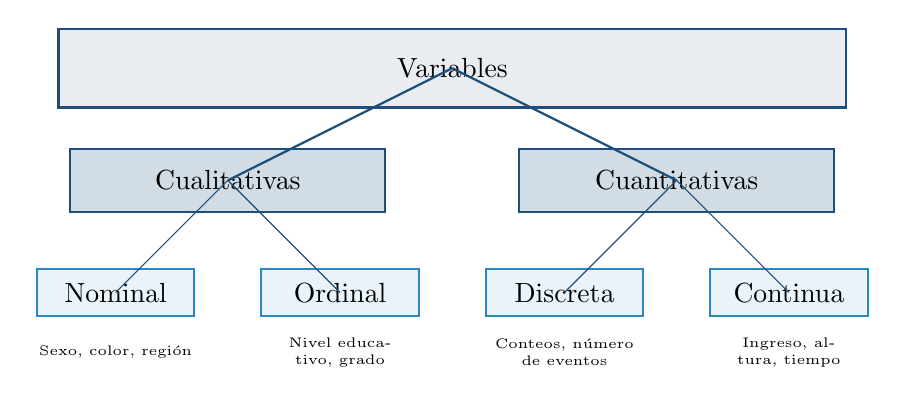
\begin{tikzpicture}[scale=0.95]
    \node[rectangle, draw=uddblue, fill=uddblue!10, thick, minimum width=10cm, minimum height=1cm] at (0,0) {Variables};

    % Left branch: Cualitativas
    \node[rectangle, draw=uddblue, fill=uddblue!20, thick, minimum width=4cm, minimum height=0.8cm] at (-3,-1.5) {Cualitativas};
    \draw[uddblue, thick] (0,0) -- (-3,-1.5);

    % Nominal
    \node[rectangle, draw=uddlight, fill=uddlight!10, thick, minimum width=2cm, minimum height=0.6cm] at (-4.5,-3) {Nominal};
    \draw[uddblue] (-3,-1.5) -- (-4.5,-3);
    \node[text width=2cm, font=\tiny, align=center] at (-4.5,-3.8) {Sexo, color, región};

    % Ordinal
    \node[rectangle, draw=uddlight, fill=uddlight!10, thick, minimum width=2cm, minimum height=0.6cm] at (-1.5,-3) {Ordinal};
    \draw[uddblue] (-3,-1.5) -- (-1.5,-3);
    \node[text width=2cm, font=\tiny, align=center] at (-1.5,-3.8) {Nivel educativo, grado};

    % Right branch: Cuantitativas
    \node[rectangle, draw=uddblue, fill=uddblue!20, thick, minimum width=4cm, minimum height=0.8cm] at (3,-1.5) {Cuantitativas};
    \draw[uddblue, thick] (0,0) -- (3,-1.5);

    % Discreta
    \node[rectangle, draw=uddlight, fill=uddlight!10, thick, minimum width=2cm, minimum height=0.6cm] at (1.5,-3) {Discreta};
    \draw[uddblue] (3,-1.5) -- (1.5,-3);
    \node[text width=2cm, font=\tiny, align=center] at (1.5,-3.8) {Conteos, número de eventos};

    % Continua
    \node[rectangle, draw=uddlight, fill=uddlight!10, thick, minimum width=2cm, minimum height=0.6cm] at (4.5,-3) {Continua};
    \draw[uddblue] (3,-1.5) -- (4.5,-3);
    \node[text width=2cm, font=\tiny, align=center] at (4.5,-3.8) {Ingreso, altura, tiempo};
  \end{tikzpicture}
\end{center}

\vspace{0.3cm}
\textit{Nota: Si disponible, ver figura `tipos_variables.pdf` en el directorio de figuras}
\end{frame}

% ============================================================================
% SLIDE 6: EJEMPLOS DE CIENCIAS SOCIALES
% ============================================================================
\begin{frame}[fragile]
\frametitle{Ejemplos en Investigación Social}
\tiny

\begin{block}{Encuesta de bienestar}
  \begin{itemize}
    \item Nominal: estado laboral
    \item Ordinal: satisfacción
    \item Discreta: años educación
    \item Continua: ingreso
  \end{itemize}
\end{block}

\pause

\begin{block}{Red social y polarización}
  \begin{itemize}
    \item Nominal: ideología
    \item Ordinal: escala ideológica
    \item Discreta: conexiones
    \item Continua: índice polarización
  \end{itemize}
\end{block}

\pause

\begin{alertblock}{Implicación analítica}
  La correcta clasificación determina la técnica: mediana para ordinal, media para continua.
\end{alertblock}
\end{frame}

% ============================================================================
% SLIDE 7: MEDIDAS DE TENDENCIA CENTRAL - INTRODUCCIÓN
% ============================================================================
\begin{frame}[fragile]
\frametitle{Medidas de Tendencia Central: Conceptos}

\begin{exampleblock}{¿Qué son?}
  Estadísticos que representan el ``centro'' o ``valor típico'' de un conjunto de datos.
\end{exampleblock}

\pause

\begin{columns}[T]
  \column{0.33\textwidth}
  \begin{block}{Media ($\bar{x}$)}
    Promedio aritmético
    $$\bar{x} = \frac{1}{n}\sum_{i=1}^{n} x_i$$
  \end{block}

  \column{0.33\textwidth}
  \begin{block}{Mediana}
    Valor central cuando datos están ordenados
    \begin{itemize}
      \item $n$ impar: valor central
      \item $n$ par: promedio dos valores centrales
    \end{itemize}
  \end{block}

  \column{0.33\textwidth}
  \begin{block}{Moda}
    Valor más frecuente
    \begin{itemize}
      \item Puede no existir
      \item Puede haber múltiples
    \end{itemize}
  \end{block}
\end{columns}
\end{frame}

% ============================================================================
% SLIDE 8: PROPIEDADES Y COMPARACIÓN
% ============================================================================
\begin{frame}[fragile]
\frametitle{Propiedades y Comparación}

\begin{table}
\small
\begin{tabular}{lccc}
\toprule
\textbf{Propiedad} & \textbf{Media} & \textbf{Mediana} & \textbf{Moda} \\
\midrule
Nivel de medición mínimo & Cuantitativo & Ordinal & Cualquier nivel \\
Utiliza todos los datos & Sí & No & No \\
Sensible a outliers & Muy & Poco & No \\
Única en un dataset & Siempre & Casi siempre & No necesariamente \\
Fácil de calcular & Sí & Sí & Sí \\
\bottomrule
\end{tabular}
\end{table}

\pause

\begin{exampleblock}{Recomendaciones de uso}
  \begin{itemize}
    \item \textbf{Media}: datos simétricos, distribuidos normalmente
    \item \textbf{Mediana}: datos sesgados, presencia de outliers (ej: ingresos)
    \item \textbf{Moda}: datos categóricos, interés en categoría más frecuente
  \end{itemize}
\end{exampleblock}
\end{frame}

% ============================================================================
% SLIDE 9: SENSIBILIDAD A OUTLIERS
% ============================================================================
\begin{frame}[fragile]
\frametitle{Sensibilidad a Outliers: Ejemplo Numérico}
\small

\begin{block}{Dataset de ingresos (UF)}
  \textbf{Sin outliers:} 2.0, 2.2, 2.5, 2.8, 3.1, 3.3, 3.5
  \begin{itemize}
    \item Media: 2.77 UF | Mediana: 2.8 UF
  \end{itemize}

  \pause
  \vspace{0.15cm}
  \textbf{Con outlier:} 2.0, 2.2, 2.5, 2.8, 3.1, 3.3, 3.5, 500.0
  \begin{itemize}
    \item Media: 64.85 UF ← \textcolor{red}{cambia drásticamente}
    \item Mediana: 2.95 UF ← sigue siendo representativa
  \end{itemize}
\end{block}

\pause

\begin{alertblock}{Conclusión para ciencias sociales}
  \small Con datos sesgados (ingresos, riqueza), \textbf{mediana} > media
\end{alertblock}
\end{frame}

% ============================================================================
% SLIDE 10: MEDIDAS DE DISPERSIÓN - INTRODUCCIÓN
% ============================================================================
\begin{frame}[fragile]
\frametitle{Medidas de Dispersión}

\begin{exampleblock}{¿Por qué las necesitamos?}
  Dos datasets pueden tener la misma media pero dispersiones muy distintas:

  \begin{itemize}
    \item \textbf{Grupo A}: 2.5, 2.5, 2.5, 2.5, 2.5 $\Rightarrow$ Media = 2.5, Desv = 0
    \item \textbf{Grupo B}: 1.0, 2.0, 2.5, 3.0, 4.0 $\Rightarrow$ Media = 2.5, Desv = 1.12
  \end{itemize}

  Las medidas de dispersión cuantifican esta variabilidad.
\end{exampleblock}

\pause

\begin{block}{Medidas principales}
  \begin{itemize}
    \item Rango (máximo - mínimo)
    \item Varianza y Desviación Estándar
    \item Rango Intercuartílico (IQR)
    \item Coeficiente de Variación
  \end{itemize}
\end{block}
\end{frame}

% ============================================================================
% SLIDE 11: VARIANZA Y DESVIACIÓN ESTÁNDAR
% ============================================================================
\begin{frame}[fragile]
\frametitle{Varianza y Desviación Estándar}
\small

\begin{block}{Varianza}
  $$s^2 = \frac{1}{n-1} \sum_{i=1}^{n} (x_i - \bar{x})^2$$
  Unidades al cuadrado; difícil de interpretar
\end{block}

\pause

\begin{block}{Desviación Estándar}
  $$s = \sqrt{\frac{1}{n-1} \sum_{i=1}^{n} (x_i - \bar{x})^2}$$
  Mismas unidades; desviación promedio desde media
\end{block}

\pause

\begin{alertblock}{Regla empírica}
  68\% dentro $[\bar{x} \pm s]$; 95\% dentro $[\bar{x} \pm 2s]$
\end{alertblock}
\end{frame}

% ============================================================================
% SLIDE 12: RANGO INTERCUARTÍLICO Y CUARTILES
% ============================================================================
\begin{frame}[fragile]
\frametitle{Cuartiles y Rango Intercuartílico}
\small

\begin{block}{Cuartiles}
  \begin{itemize}
    \item $Q_1$: percentil 25
    \item $Q_2$: percentil 50 (mediana)
    \item $Q_3$: percentil 75
  \end{itemize}
\end{block}

\begin{block}{Rango Intercuartílico (IQR)}
  $$\text{IQR} = Q_3 - Q_1$$
  50\% central; robusto a outliers
\end{block}

\pause

\begin{alertblock}{Outliers (método IQR)}
  Fuera $[Q_1 - 1.5 \times \text{IQR}, Q_3 + 1.5 \times \text{IQR}]$
\end{alertblock}
\end{frame}

% ============================================================================
% SLIDE 13: COEFICIENTE DE VARIACIÓN
% ============================================================================
\begin{frame}[fragile]
\frametitle{Coeficiente de Variación (CV)}

\begin{block}{Coeficiente de Variación (CV)}
  $$\text{CV} = \frac{s}{\bar{x}} \times 100\%$$

  \begin{itemize}
    \item Dispersión \textbf{relativa} (no absoluta)
    \item Permite comparar variabilidad entre variables con distintas escalas
    \item Ejemplo: comparar dispersión de ingresos vs. educación
    \item CV alto: datos muy dispersos respecto a la media
    \item Permite comparación entre variables
  \end{itemize}
\end{block}

\pause

\begin{exampleblock}{Interpretación}
  Si CV$_{\text{ingresos}} = 45\%$ y CV$_{\text{educación}} = 30\%$, los ingresos tienen mayor variabilidad relativa.
\end{exampleblock}
\end{frame}

% ============================================================================
% SLIDE 13b: Z-SCORES (ESTANDARIZACIÓN)
% ============================================================================
\begin{frame}[fragile]
\frametitle{Z-Scores (Estandarización)}

\begin{block}{Z-Scores}
  $$z_i = \frac{x_i - \bar{x}}{s}$$

  \begin{itemize}
    \item Transforma datos a media 0, desv. est. 1
    \item Interpretación: ``cuántas desviaciones estándar del promedio''
    \item Permite comparación entre variables con escalas distintas
    \item Identificar valores inusuales: $|z| > 3$ es potencial outlier
  \end{itemize}
\end{block}

\pause

\begin{exampleblock}{Ejemplo}
  Si ingreso medio es 3 UF con s = 0.5, una persona con 4.5 UF tiene:
  $$z = \frac{4.5 - 3}{0.5} = 3 \text{ (3 desviaciones estándar arriba de la media)}$$
\end{exampleblock}
\end{frame}

% ============================================================================
% SLIDE 14: VISUALIZACIÓN EN R - CARGA DE DATOS
% ============================================================================
\begin{frame}[fragile]
\frametitle{Implementación en R: Cargar y Resumir Datos}

\begin{lstlisting}[basicstyle=\ttfamily\tiny]
library(tidyverse)
library(ggplot2)
datos <- read.csv("datos_encuesta.csv")
str(datos)
head(datos)
datos %>% summarise(
  media = mean(ingreso, na.rm = TRUE),
  mediana = median(ingreso, na.rm = TRUE),
  desv_est = sd(ingreso, na.rm = TRUE),
  q1 = quantile(ingreso, 0.25),
  q3 = quantile(ingreso, 0.75)
)
\end{lstlisting}
\end{frame}

% ============================================================================
% SLIDE 15: VISUALIZACIÓN CON GGPLOT2 - HISTOGRAMAS
% ============================================================================
\begin{frame}[fragile]
\frametitle{Visualización: Histogramas de Ingresos}

\begin{lstlisting}[basicstyle=\ttfamily\tiny]
ggplot(datos, aes(x = ingreso)) +
  geom_histogram(binwidth = 0.5,
    fill = "#2E86C1", color = "white") +
  labs(title = "Income Distribution",
       x = "Income (UF)", y = "Frequency") +
  theme_minimal()
ggplot(datos, aes(x = ingreso)) +
  geom_histogram(aes(y = after_stat(density)),
    binwidth = 0.5, fill = "#2E86C1") +
  geom_density(color = "#1F4E79") +
  theme_minimal()
\end{lstlisting}

\textit{Nota: Ver figura `histograma_ingresos.pdf`}
\end{frame}

% ============================================================================
% SLIDE 16: VISUALIZACIÓN CON GGPLOT2 - BOXPLOTS
% ============================================================================
\begin{frame}[fragile]
\frametitle{Visualización: Boxplots Comparativos}

\begin{lstlisting}[basicstyle=\ttfamily\tiny]
ggplot(datos, aes(x = sector, y = ingreso,
                  fill = sector)) +
  geom_boxplot(alpha = 0.7) +
  geom_jitter(width = 0.2, alpha = 0.3) +
  labs(title = "Income by Sector",
       x = "Sector", y = "Income (UF)",
       fill = "Sector") +
  theme_minimal()
ggplot(datos, aes(x = sector, y = ingreso)) +
  geom_boxplot(fill = "#2E86C1") +
  coord_flip() + theme_minimal()
\end{lstlisting}

\vspace{0.3cm}
\textit{Nota: Ver figura `boxplot_comparativo.pdf` para ejemplo real}
\end{frame}

% ============================================================================
% SLIDE 17: VISUALIZACIÓN CON GGPLOT2 - SCATTER PLOTS
% ============================================================================
\begin{frame}[fragile]
\frametitle{Visualización: Relación entre Variables}

\begin{lstlisting}[basicstyle=\ttfamily\tiny]
ggplot(datos, aes(x = education_years,
  y = income, color = gender)) +
  geom_point(size = 2.5, alpha = 0.6) +
  geom_smooth(method = "lm", se = TRUE) +
  labs(title = "Education vs Income",
       x = "Years", y = "Income (UF)",
       color = "Gender") +
  theme_minimal()
\end{lstlisting}

\textit{Nota: Ver figura `scatter_educacion_ingreso.pdf` para ejemplo real}
\end{frame}

% ============================================================================
% SLIDE 18: RESUMEN DE ESTADÍSTICOS EN R
% ============================================================================
\begin{frame}[fragile]
\frametitle{Tabla Resumida de Estadísticos por Grupo}

\begin{lstlisting}[basicstyle=\ttfamily\tiny]
resumen <- datos %>%
  group_by(sector) %>%
  summarise(
    n = n(),
    media = mean(ingreso),
    mediana = median(ingreso),
    sd = sd(ingreso),
    cv = (sd / media) * 100,
    min = min(ingreso),
    max = max(ingreso)
  )
print(resumen)
\end{lstlisting}
\end{frame}

% ============================================================================
% SLIDE 19: OUTLIERS Y DATOS ANÓMALOS
% ============================================================================
\begin{frame}[fragile]
\frametitle{Identificación y Manejo de Outliers}

\begin{lstlisting}[basicstyle=\ttfamily\tiny]
datos <- datos %>%
  mutate(z_ingreso = scale(ingreso)[,1],
         es_outlier = abs(z_ingreso) > 3)
ggplot(datos, aes(x = "Ingreso", y = ingreso)) +
  geom_boxplot(fill = "#2E86C1", alpha = 0.5) +
  geom_point(aes(color = es_outlier),
    size = 3, alpha = 0.7) +
  theme_minimal()
tabla_outliers <- datos %>%
  summarise(
    total = n(),
    outliers = sum(es_outlier),
    pct = (sum(es_outlier) / n()) * 100)
\end{lstlisting}
\end{frame}

% ============================================================================
% SLIDE 20: TRANSFORMACIONES DE DATOS
% ============================================================================
\begin{frame}[fragile]
\frametitle{Transformaciones: Normalizando Datos Sesgados}
\small

\begin{exampleblock}{Problema}
  Ingresos y riqueza: distribuciones fuertemente sesgadas
\end{exampleblock}

\begin{lstlisting}[basicstyle=\ttfamily\tiny]
datos <- datos %>%
  mutate(log_income = log(income),
         sqrt_income = sqrt(income))
p1 <- ggplot(datos, aes(x = income)) +
  geom_histogram(fill = "#2E86C1") +
  ggtitle("Original")
p2 <- ggplot(datos, aes(x = log_income)) +
  geom_histogram(fill = "#2E86C1") +
  ggtitle("Log Transformed")
grid.arrange(p1, p2, ncol = 2)
\end{lstlisting}
\end{frame}

% ============================================================================
% SLIDE 21: DISTRIBUCIONES BIVARIADAS
% ============================================================================
\begin{frame}[fragile]
\frametitle{Correlación entre Variables}
\small

\begin{block}{Pearson: $r = \frac{\sum (x_i - \bar{x})(y_i - \bar{y})}{(n-1) s_x s_y}$}
  Rango $[-1, +1]$; mide relación lineal
\end{block}

\begin{lstlisting}[basicstyle=\ttfamily\tiny]
corr <- cor(datos$education, datos$income)
corr_mat <- cor(datos[c("age", "education",
                        "income")])
library(corrplot)
corrplot(corr_mat, method = "circle")
\end{lstlisting}
\end{frame}

% ============================================================================
% SLIDE 22: ANÁLISIS POR SUBGRUPOS
% ============================================================================
\begin{frame}[fragile]
\frametitle{Análisis Estratificado por Subgrupos}
\small

\begin{exampleblock}{Pregunta}
  ¿Cómo varían ingresos por género, región y sector?
\end{exampleblock}

\begin{lstlisting}[basicstyle=\ttfamily\tiny]
datos %>%
  group_by(gender, region, sector) %>%
  summarise(n = n(),
    mean_income = mean(income),
    med_income = median(income),
    sd_income = sd(income))
ggplot(datos, aes(x = gender, y = income,
                  fill = region)) +
  geom_boxplot(alpha = 0.7) +
  facet_wrap(~ sector)
\end{lstlisting}
\end{frame}

% ============================================================================
% SLIDE 23: BRECHA DE INGRESOS - CASO PRÁCTICO (Cálculo)
% ============================================================================
\begin{frame}[fragile]
\frametitle{Caso Práctico: Análisis de Brecha de Género (Cálculo)}

\begin{exampleblock}{Calculate wage gap}
  \begin{lstlisting}[basicstyle=\ttfamily\tiny]
datos %>%
  group_by(gender) %>%
  summarise(mean_income = mean(income),
    median_income = median(income))
gap <- datos %>%
  group_by(gender) %>%
  summarise(mean = mean(income)) %>%
  pivot_wider(names_from = gender,
              values_from = mean) %>%
  mutate(gap_pct = ((Female -
    Male) / Male) * 100)
  \end{lstlisting}
\end{exampleblock}
\end{frame}

% ============================================================================
% SLIDE 23b: BRECHA DE INGRESOS - VISUALIZACIÓN
% ============================================================================
\begin{frame}[fragile]
\frametitle{Caso Práctico: Análisis de Brecha de Género (Visualización)}

\begin{exampleblock}{Visualizar}
  \begin{lstlisting}[basicstyle=\ttfamily\tiny]
ggplot(datos, aes(x = gender, y = income,
                  fill = gender)) +
  geom_violin(alpha = 0.6) +
  geom_boxplot(width = 0.1, fill = "white") +
  labs(title = "Income Distribution by Gender",
       x = "Gender", y = "Income (UF)") +
  theme_minimal()
  \end{lstlisting}
\end{exampleblock}

\pause

\begin{alertblock}{Interpretación}
  La mediana y cuartiles muestran si la brecha es real más allá de valores extremos.
\end{alertblock}
\end{frame}

% ============================================================================
% SLIDE 24: ASIMETRÍAS Y SESGO
% ============================================================================
\begin{frame}[fragile]
\frametitle{Simetría y Sesgo}
\tiny

\begin{columns}[T]
  \column{0.5\textwidth}
  \begin{block}{Sesgo}
    = 0: simétrica \\
    > 0: derecha \\
    < 0: izquierda
  \end{block}

  \column{0.5\textwidth}
  \begin{block}{Ejemplos}
    Ingresos > 0 \\
    Jubilación < 0
  \end{block}
\end{columns}

\vspace{-0.1cm}
\pause

\begin{lstlisting}[basicstyle=\ttfamily\tiny]
library(moments)
sesgo <- skewness(datos$ingreso)
ggplot(datos, aes(x = ingreso)) +
  geom_histogram(aes(y = after_stat(density)),
    fill = "#2E86C1") +
  geom_density(color = "#1F4E79")
\end{lstlisting}
\end{frame}

% ============================================================================
% SLIDE 25: CHECKLIST DE ANÁLISIS DESCRIPTIVO
% ============================================================================
\begin{frame}[fragile]
\frametitle{Checklist: Análisis Descriptivo Completo}

\begin{alertblock}{Antes de cualquier análisis inferencial, verificar:}
  \begin{itemize}
    \item[\checkmark] \textbf{Estructura del dataset}: dimensiones, tipos de datos, valores faltantes
    \item[\checkmark] \textbf{Tendencia central}: media, mediana, moda (¿cuál es representativa?)
    \item[\checkmark] \textbf{Dispersión}: desv. estándar, IQR, rango (¿cuán concentrados están datos?)
    \item[\checkmark] \textbf{Forma}: simetría, sesgo, curtosis (¿es aproximadamente normal?)
    \item[\checkmark] \textbf{Outliers}: detectar y evaluar si son reales o errores
    \item[\checkmark] \textbf{Distribuciones por grupo}: ¿hay patrones por subgrupos?
    \item[\checkmark] \textbf{Relaciones bivariadas}: correlaciones entre pares de variables
    \item[\checkmark] \textbf{Valores faltantes}: ¿cuántos?, ¿patrón?, ¿imputar o eliminar?
  \end{itemize}
\end{alertblock}

\pause

\begin{block}{Salida de una buena estadística descriptiva}
  Una tabla o gráfico que comunique hallazgos clave de forma clara y honesta.
\end{block}
\end{frame}

% ============================================================================
% SLIDE 26: EJERCICIO PRÁCTICO
% ============================================================================
\begin{frame}[fragile]
\frametitle{Exercise: 30 min}
\tiny

\begin{block}{Instructions}
  \begin{itemize}
    \item Load survey data
    \item Compute 5 descriptive stats
    \item Create 3 visualizations
    \item Compare by gender
    \item Identify best predictor
  \end{itemize}
\end{block}
\end{frame}

% ============================================================================
% SLIDE 27: ERRORES COMUNES A EVITAR (Parte 1)
% ============================================================================
\begin{frame}[fragile]
\frametitle{Errores Comunes}
\small

\begin{alertblock}{Evitar:}
  \begin{itemize}
    \item Media sin verificar simetría
    \item Ignorar outliers
    \item Ordinal como continua
    \item Olvidar tamaño muestral
    \item Correlación como causalidad
  \end{itemize}
\end{alertblock}

\pause

\begin{block}{Por qué}
  Media + sesgo = engaño; Outliers = incompleto; Escalas = técnicas malas
\end{block}
\end{frame}

% ============================================================================
% SLIDE 27b: BUENAS PRÁCTICAS
% ============================================================================
\begin{frame}[fragile]
\frametitle{Buenas Prácticas en Estadística Descriptiva}

\begin{block}{Lo que \textbf{SÍ} debes hacer:}
  \begin{itemize}
    \item \checkmark Reportar \textbf{múltiples} medidas de tendencia central
    \item \checkmark Justificar decisiones sobre outliers
    \item \checkmark Incluir visualizaciones para cada variable importante
    \item \checkmark Documentar el proceso y decisiones tomadas
    \item \checkmark Ser transparente sobre limitaciones y supuestos
    \item \checkmark Crear gráficos con títulos y etiquetas claros
  \end{itemize}
\end{block}

\pause

\begin{exampleblock}{Checklist antes de reportar}
  ¿He descrito la muestra? ¿He verificado supuestos? ¿Las conclusiones son respaldadas por los datos?
\end{exampleblock}
\end{frame}

% ============================================================================
% SLIDE 28: RECURSOS Y REFERENCIAS
% ============================================================================
\begin{frame}[fragile]
\frametitle{Referencias}
\small

\begin{block}{Libros}
  \begin{itemize}
    \item Agresti (2018): Statistical Methods
    \item Wickham \& Grolemund (2016): R for Data Science
    \item Field (2013): Discovering Statistics Using R
  \end{itemize}
\end{block}

\begin{block}{Paquetes R}
  \begin{itemize}
    \item \texttt{tidyverse}: datos
    \item \texttt{ggplot2}: gráficos
    \item \texttt{psych}: descriptivos
    \item \texttt{corrplot}: correlaciones
  \end{itemize}
\end{block}
\end{frame}

% ============================================================================
% SLIDE 28b: RECURSOS ONLINE
% ============================================================================
\begin{frame}[fragile]
\frametitle{Recursos Online}
\small

\begin{block}{Documentación}
  \begin{itemize}
    \item \url{https://r4ds.had.co.nz} — R for Data Science
    \item \url{https://ggplot2.tidyverse.org} — ggplot2
    \item \url{https://www.r-bloggers.com} — Tutoriales
  \end{itemize}
\end{block}
\end{frame}

% ============================================================================
% SLIDE 29: RESUMEN DE SESIÓN
% ============================================================================
\begin{frame}[fragile]
\frametitle{Resumen de Sesión 1}
\small

\begin{exampleblock}{Temas cubiertos:}
  \begin{enumerate}
    \item Tipos de datos y escalas
    \item Tendencia central
    \item Dispersión
    \item Visualización con ggplot2
    \item Implementación en R
    \item Aplicaciones prácticas
  \end{enumerate}
\end{exampleblock}

\pause

\begin{alertblock}{Mensaje clave}
  \textbf{La estadística descriptiva es fundamental}. Entiende tus datos antes de inferir.
\end{alertblock}

\pause

\begin{block}{Próxima sesión}
  Probabilidad y distribuciones
\end{block}
\end{frame}

% ============================================================================
% SLIDE 30: PREGUNTAS
% ============================================================================
\begin{frame}[fragile]
\frametitle{¿Preguntas?}

\vspace{2cm}

\begin{center}
  \Large
  \textbf{¡Gracias por su atención!}

  \vspace{1cm}

  \normalsize
  Amaru Agüero \\
  \texttt{a.agueroj@udd.cl}

  \vspace{1cm}

  \textit{Doctorado en Ciencias de la Complejidad Social — CICS, UDD}
\end{center}

\end{frame}

\end{document}
